\documentclass{homework}
\author{王褕立}
\title{\LaTeX 作業模板}

\begin{document}
\maketitle

\section{數學式}

\begin{enumerate}[1.]
	\item 用星號代替 \verb|\cdot| ,例如 \verb|$a * b = c$| 會產生 $a * b = c$ 。需要星號請用  \verb|\ast| 。\\
	\item \verb|$\abs{a}, \ceil{n}, \floor{n}, \inner{n}, \norm{n}, \set{n}, \Set{n}$|\\
		會產生$\abs{a}, \ceil{n}, \floor{n}, \inner{n}, \norm{n}, \set{n}, \Set{n}$。加星號可以取消自動縮放括號。
	\item $\N, \Z, \Q, \R, \C$| 會產生 $\N, \Z, \Q, \R, \C$ ,不需要 \verb|\mathbb|。
	\item \verb|$\contra, \oiint, \iiint, \mathbat, \underleftflutteringbat{abc \ldots z}$| 會產生 $\contra, \oiint, \iiint, \mathbat, \underleftflutteringbat{abc \ldots z}$
\end{enumerate}

範例:
\[
	\abs{\frac{1}{1 - \lambda h}} \le 1
	\qquad\text{and}\qquad
	\bigcup_{i=1}^n \; \set{z \in \C \mid \abs*{z - a_{ii}} \le {\sum\nolimits_{j \ne i}} \abs*{a_{ij}}}.
\]

\section{方塊們}

\begin{corollary}[推論 Corollary]
	推推推推推推推推推推
\end{corollary}

\begin{lemma}[引理 Lemma]
	引引引\emph{引引引引}引引引
\end{lemma}

\begin{theorem}[定理 Theorem]
	定定\emph{定定定定}定定定定
\end{theorem}

\begin{definition}[定義 Definition]
	定定定定定定定定定定
\end{definition}

\begin{observation}[觀察 Observation]
	觀觀觀觀觀觀觀觀觀觀
\end{observation}

\section{題目}

題目會和 Section 共用 counter 的樣子,所以建議用中括號自己打題號。

\problem*
除了第一題,其餘每一題都會自動放在新的一頁。如果想要連接上文,請用加了星號的版本 \verb|\problem*| 。

\problem*[Rec--2.1]
你也可以自己設定題號 \dots

\setcounter{problem}{7}
\problem*
\dots 或是用 \verb|\setcounter{problem}{x}| 跳過一些號碼。

\setcounter{section}{3}

\section{程式碼}

行內的話可以用 \verb|\texttt|,效果像這樣:\texttt{std::cout << "Hello world!" << std::endl;} 。
或是可以用 \verb|\mintinline|,效果像這樣:\mintinline{c++}{std::cout << "Hello world!" << std::endl;} 。

你也可以用 \verb|\Code| 來插入程式碼:

\Code[firstline=2,lastline=15]{files/example.cpp}

這個指令只支援 C 和 C++ ,其他語言請自行使用 \verb|\inputminted| 。

底下是 psuedo-code 範例:

\begin{algorithm}[H]
	\caption{PPO}
	\label{alg:ppo}
	\begin{algorithmic}[1]
		\For {$iteration=1,2,\ldots$}
		\For {$actor=1,2,\ldots,N$}
		\State Run policy $\pi_{\theta_{old}}$ in environment for $T$ time steps
		\State Compute advantage estimates $\hat{A}_{1},\ldots,\hat{A}_{T}$
		\EndFor
		\State Optimize surrogate $L$ wrt. $\theta$, with $K$ epochs and minibatch size $M\leq NT$
		\State $\theta_{old}\leftarrow\theta$
		\EndFor
	\end{algorithmic}
\end{algorithm}

\section{插入圖片}

\begin{figure}[htpb]
	\centering
	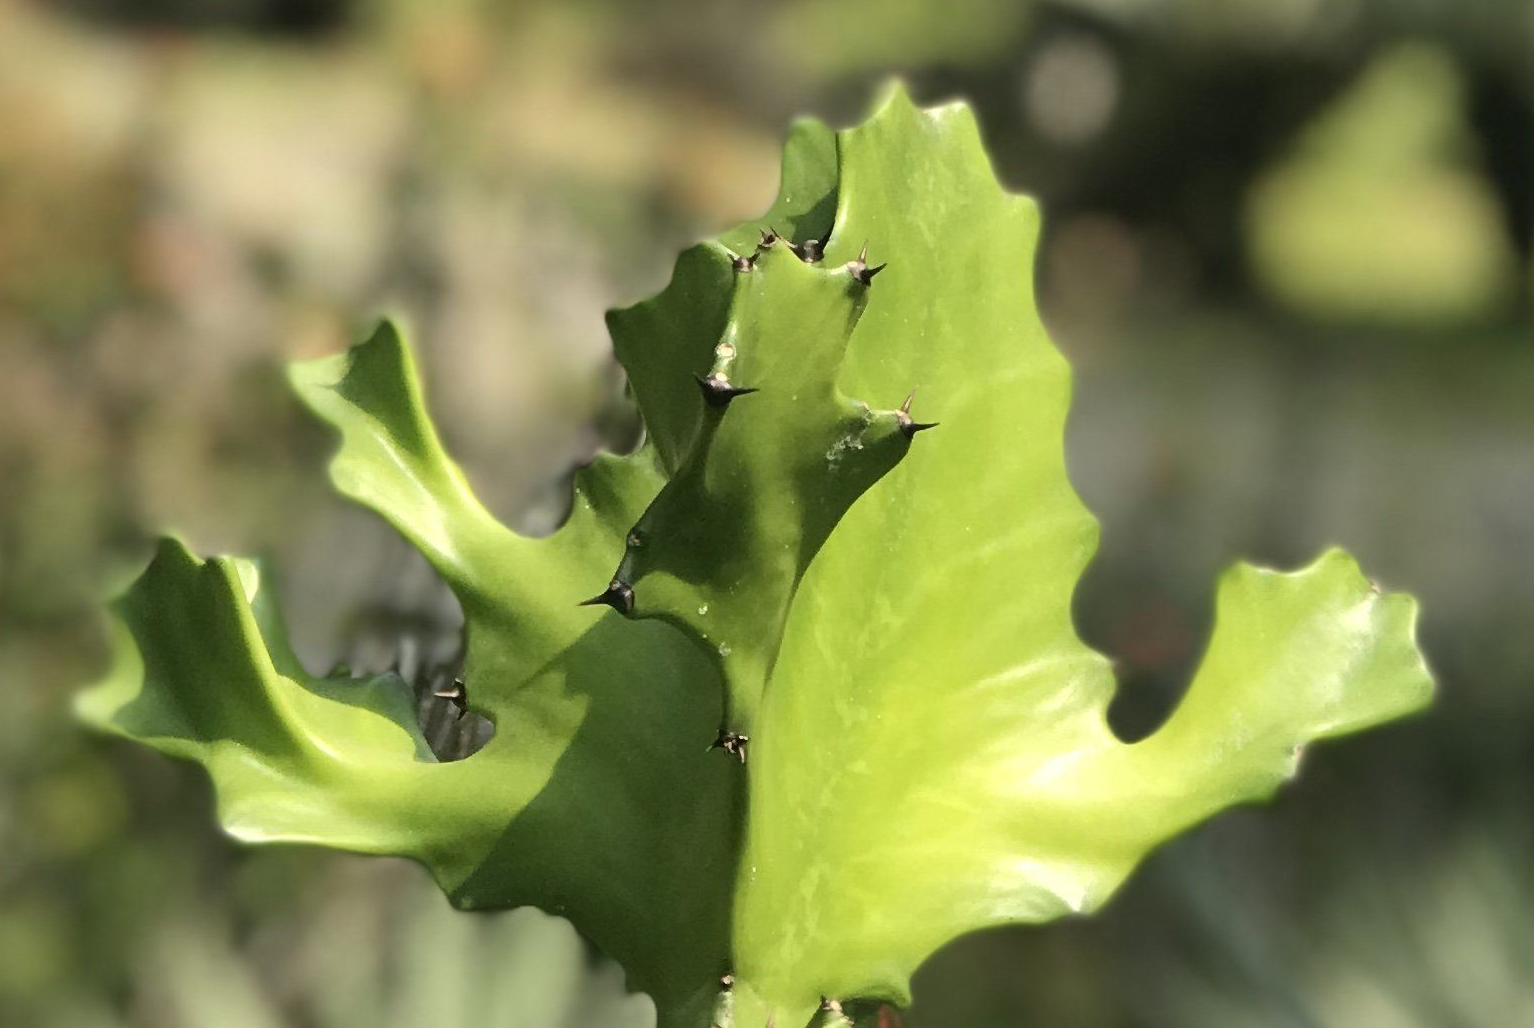
\includegraphics[width=0.8\textwidth]{files/cactus.jpeg}
	\caption{仙人掌}
	\label{fig:cactus}
\end{figure}

你也可以用 \verb|\ref| 來連結圖片或圖表,例如:圖片 \ref{fig:cactus} 和演算法 \ref{alg:ppo} 。

\section{超連結}

可以直接用連結 \url{https://youtu.be/EeA_Y0FSv5Q} 或是 \href{https://youtu.be/EeA_Y0FSv5Q}{自訂文字} 。

\end{document}
